\documentclass[12pt]{article}

\usepackage[a4paper, total={7in, 9.5in}]{geometry}
\usepackage{array}
\usepackage{graphicx}

\begin{document}

\begin{centering}
    {\large 15-418 Parallel Computer Arch., Spring 2021\\}
    \vspace{2ex}
    {\LARGE Parallel Boids Project Checkpoint\\}
    \vspace{2ex}
    {\large Due Date: Friday April 26, 2021 22:59 EST\\}
\end{centering}

\bigskip

\paragraph{Group:} Elan Biswas (elanb), Gustavo Silvera (gsilvera)

\section*{New Project:} 
\par After further investigation of our original proposal \textit{(parallel phase-based video interpolation)} we have decided that it would be more beneficial to focus on a project that has a lower barrier-of-entry. Neither of our group members felt comfortable with the complex material covered in the video interpolation papers, and we would need to spend most of the time on this project understanding the algorithms (as well as implementing heavy linear algebra operations) before even reaching the parellellization aspect of the paper which we believe should be the focus of our project.
\par To that end, we've decided to switch projects to a nature-based simulation. In particular, we are interested in simulating ``swarm behaviour'' as defined through the Boids algorithm with a focus on various parallel work schemes (\texttt{https://en.wikipedia.org/wiki/Boids}). 
\par As some quick background, the Boids algorithm was developed by Craig Reynolds in 1986 as a method to simulate flocking behaviour as seen in nature. This can be applied to birds, fish, insects, and even swarm robotics. The Boids algorithm follows three relatively simple rules to control each agent in the flock: Cohesion, Separation, and Alignment.:
\par \textbf{Cohesion} is used to drive every boid in the flock to the ``center of mass'' of their flock.
\par \textbf{Separation} is used to drive boids away from nearby neighbours, to avoid collisions
\par \textbf{Alignment} is used to keep all the boids matching the others' velocities (speed \& direction)\\
\par On top of the generic Boids algorithm (which you can see described in pseudocode here: \texttt{http://www.vergenet.net/{\textasciitilde}conrad/boids/pseudocode.html}) we are especially interested in the mechanics of agent (Boid) communication and particularly flocking. When dealing with ``flocks'', we'll need the simulator's agents to designate a flock leader who recruits other boids into their flock. This abstration allows us to have separate flocks each compute their own Boid swarm independently from distant flocks, providing another axis of parallelism on top of the agents themselves.
\par What we'll primarily be investigating in this project is how we can best optimize the algorithm to work with large numbers of Boids. This will be challenging because we'll need to account for the large amount of communication across Boids and will likely be memory constrained which will require optimizations in scheduling and locality to make a significant impact. We'll also investigate across various parallel architectures, CPU \& GPU, and see how the parallelism scales across them.

\newpage 
\section*{Current Progress:} 
\par So far we've built a fully functional sequential implementation of an N-body Boid simulator with support for arbitrary numbers of Boids, arbitrary image sizes (constrained by the memory on the system), and image rendering (similar to the \texttt{.ppm}'s in assignment 1) to disk which can then be packed together into a movie (such as an \texttt{.mp4}). (In fact, our GitHub repository is publically available at this link: \texttt{https://github.com/GustavoSilvera/ParallelBoids})
\par From the sequential algorithm, it is not difficult to parellelize naively across the Boids with \texttt{OpenMP}. With this in mind, we also built our first (very simple) parallel implementation of this simulator. The main uses of \texttt{OpenMP} are using a \texttt{\#pragma omp parallel for num\_threads(X)} as the main axis of parallelism across the Boids, and \texttt{\#pragma omp critical} when updating the flock information. 
\par The way we update our agents in the simulator follows the standard ``sense $\to$ plan $\to$ act'' agent-strategy where all agents \texttt{sense()}, \texttt{plan()}, and \texttt{act()} in parallel so everyone is using the same data on every \texttt{tick()}.
\begin{center}
    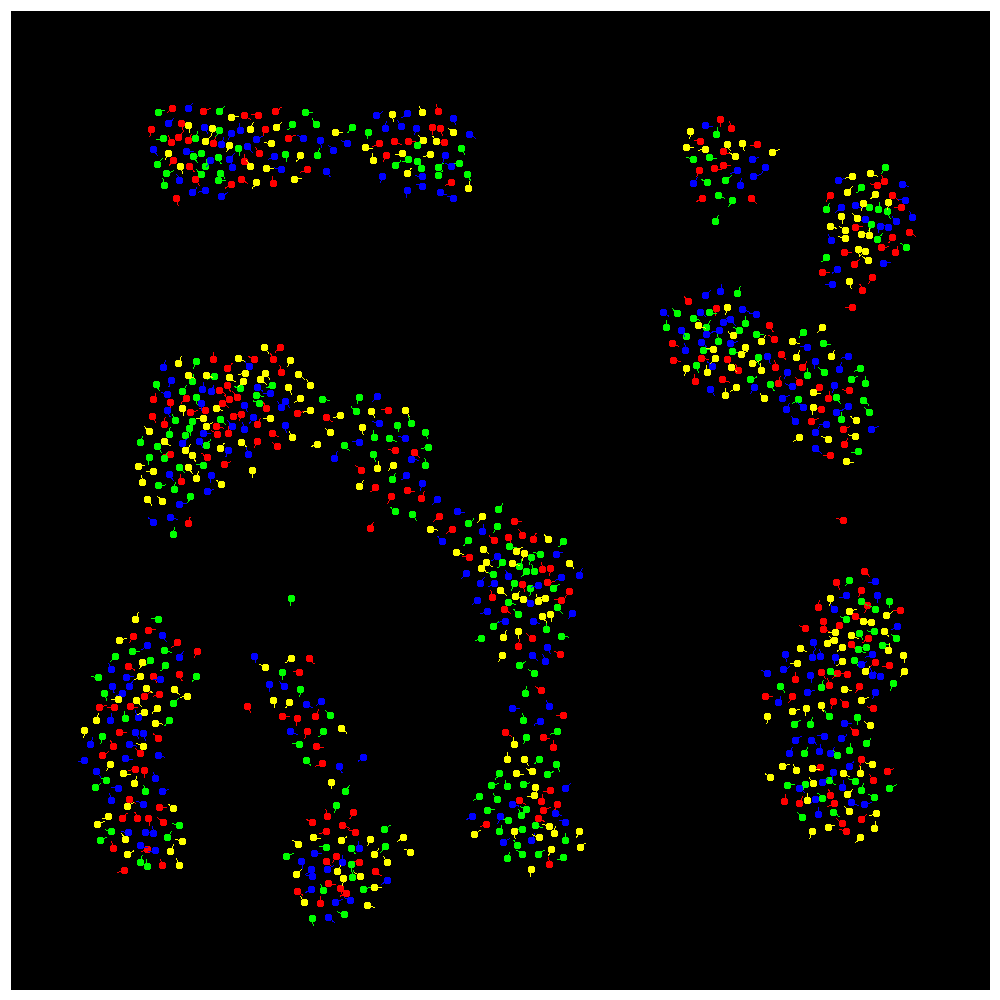
\includegraphics[width=200px]{figures/0156_procs.png}
    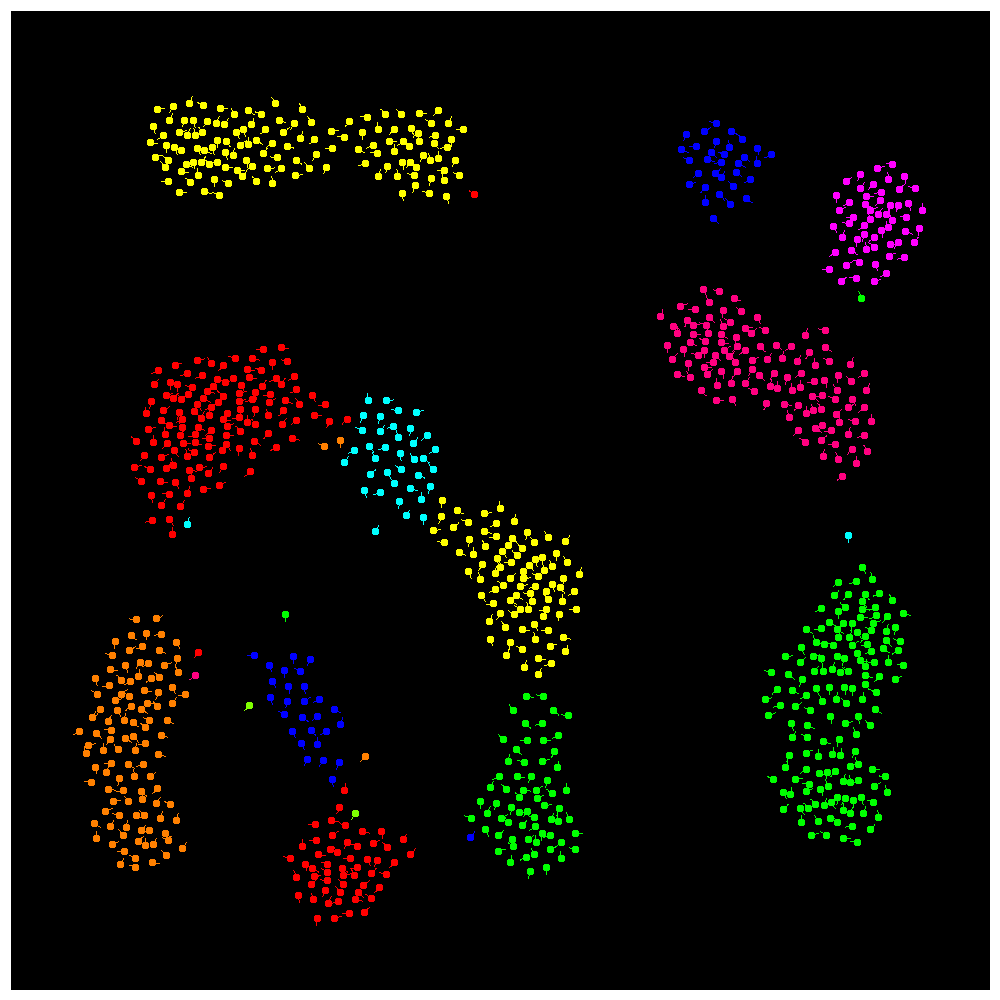
\includegraphics[width=200px]{figures/0156_flocks.png}\\
    Figure 1: Colour-labeled Boids based off thread id (left) and flock id (right)
\end{center}
\par Intuitively, we could improve locality and reduce communication across processors by having the processors assigned to flocks rather than individual Boids. As seen in the left half of Figure 1, the the agents are coloured in a uniformally randomly distributed fashion for all (in this case, 4) processors. This means that for all ``flocks'', we'll have lots of communication between all processors which can be very expensive on the shared interconnect. On the other hand, if we manage to schedule the processors and assign work based off groups of Boids (based off our ``flocks'') then all the agent updates (sensing \& planning \& acting) can greatly benefit from locality per thread. 
\par As seen with our current (simplistic) parallel implementation our speedup is not as good as we'd like, indicating that we definitely have room for improvement and bottlenecks to overcome. We see problems especially with large numbers of threads (past 8) where the speedup consistently reduces in performance. This also leads us to infer that communication is a big bottleneck across large numbers of processors as our lectures on Cache Coherence and Memory Consistency have shown us in 15-418. 
\begin{center}
    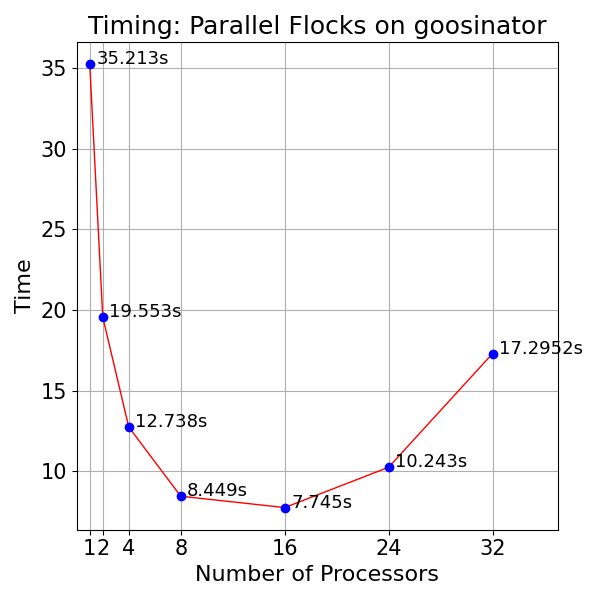
\includegraphics[width=200px]{figures/Time_ParallelFlocks_goosinator.png}
    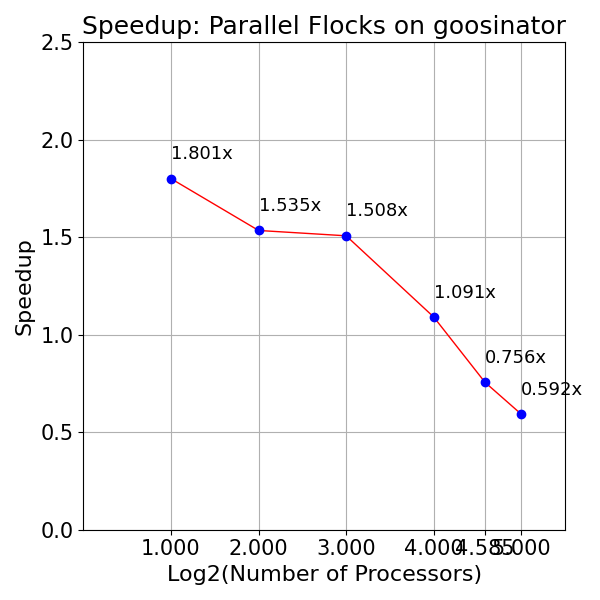
\includegraphics[width=200px]{figures/Speedup_ParallelFlocks_goosinator.png}\\
    Figure 2: Timings and speedup of our parallel Boids simulator
\end{center}
\par The above measurements were taken on the \texttt{goosinator} machine, which is \texttt{gsilvera}'s local machine which is running an AMD 3900x 12-core 24-thread CPU @ 4.00GHz. This is expected since the problem itself is not embarrassingly parallel as we have inherent communication that must be dealt with between agents and a global data structure that manages the flocks across the entire simulation.
\section*{Goals \& Deliverables:} 
We plan to implement 2 parallel versions of the Boid algorithm, one utilizing the GPU via CUDA and the other utilizing multicore processing via OMP (and later potentially MPI).
\paragraph*{Parallelization Schemes:}$~$\\
- CPU: \texttt{OpenMP} as main parallelism avenue, potentially also add \texttt{MPI} to utilize multiple machines\\
- GPU: \texttt{CUDA} on device, potentially \texttt{OpenMP} on host \\
\par For each mode of parallelism, we will experiment with different partitioning schemes (static, semi-static, dynamic) of work to the CPU/GPU based on the different flocks in the scene. If there are only a few large flocks we plan to partition based on distance from the flock's center-of-mass so that contours of Boids are parallelized over by a thread. In most cases (with large number of Boids) there should be many independent flocks that can each be assigned to a processor, with many Boids per flock, making this a good choice for GPU-based parallelism. 
\par We are currently planning to present to the class a slideshow presentation (such as Google Presentation) with graphs denoting the comparisons between our initial (simple) and complex (dynamic/flock-based) parallel implementations, highlighting which performs better and why. We could also present a visualization in movie format (such as  \texttt{.gif}) that would show the entire simulation execution of all the Boids. 
\paragraph*{Nice to have:}$~$\\
- It would also be nice to use a canvas-drawing application, such as \texttt{OpenGL} or \texttt{Cinder C++} to draw the updated frames to a refreshing window rather than as discrete images to disk. This would allow for a real-time interaction experience that could be a fun project to play with. This would be similar to this Boids example \texttt{https://eater.net/boids} where various Boid parameters are set, but the flocks don't respond to user input otherwise. \\
- It would be nice to incorporate \texttt{MPI} into our CPU-based implementation to get further performance gains when parallelizing across flocks that are completely independent from one another (such as being far apart). As is commonly done in industry, we'll focus on using \texttt{OpenMP} within a machine, and using \texttt{MPI} when segmenting the problem into independent pieces to work on other machines.\\
- Implement an approximation involving computing frames at double the time step granularity and interpolating the missing frames in between. We hypothesize that this will allow for greater parallelism while not sacrificing as much in terms of correctness. We would verify this by measuring the relative performance of the correct and approximated implementations and comparing with the loss of accuracy. Since we are limited on time, it is not likely that we will accomplish this.\\

\section*{Detailed Schedule:} 
\underline{April 26-28}
\par (Elan) - Start on GPU implementation. This includes writing the major kernels and restructuring data to be used by device code.
\par (Gus) - Continue working on the OpenMP implementation optimizations such as the dynamic flock-based work partitioning algorithm. 
\par (Both) - Take initial performance metrics and document them in the report.
\\\\
\underline{April 29-May 1}
\par (Elan) - Incorporate schemes into GPU implementation.
\par (Gus) - Incorporate schemes into OMP implementation.
\par (Both) - Implement the work partitioning schemes 
\\\\
\underline{May 2-5}
\par (Both) - Measure performance using each partition scheme and compare with previously recorded metrics in report. Continue to make improvements to both implementations.
\\\\
\underline{May 6-8}
\par (Both) - Finish both implementations, including performance optimizations and resolving any lingering bugs.
\par Record final measurements and add to report. 
\\\\
\underline{May 9-11}
\par (Both) - Formalize the report by compiling and discussing all recorded metrics. Begin work on the presentation and slideshow layout. (If we are ahead of schedule we can work on the ``nice to have'' portion involving the frame interpolation and MPI)
\\\\
\underline{May 12-13}
\par (Both) - Finalize project presentation and slide deck and wrap up any ``nice to haves'' that we may have started.

\section*{Main Concerns:} 
\par Our primary concerns stem from switching projects and getting a little behind. However, our detailed schedule is feasible and we should be able to meet our goals by the project deadline. 
\par We hypothesize that since the Boids lend themselves very naturally to SIMD execution, the CUDA implementation will far outpace the CPU-based implementation. Our primary concern in this regard is that the analysis comparing the two will not be very interesting. To compensate for this, we will also be comparing the different partitioning schemes and analyzing their effect in both environments.
\par We are also slightly concerned with mixing multiple parallel schemes together (\texttt{OpenMP + MPI}, \texttt{CUDA + OpenMP}) if we advance to some of the ``Nice to have'''s since we do not have experience with mixing them together from the course. In particular we are not sure if we want to spend time dealing with parallel kernel calls (from OpenMP host calling device code in multiple threads) in CUDA, and networking issues when communicating across computers in a network (local or not). We should still be able to figure these out, but the main concern is getting everything to work on time before the semester ends. 
\end{document}
